\documentclass[letterpaper,12pt]{article}\usepackage[]{graphicx}\usepackage[]{color}
%% maxwidth is the original width if it is less than linewidth
%% otherwise use linewidth (to make sure the graphics do not exceed the margin)
\makeatletter
\def\maxwidth{ %
  \ifdim\Gin@nat@width>\linewidth
    \linewidth
  \else
    \Gin@nat@width
  \fi
}
\makeatother

\definecolor{fgcolor}{rgb}{0.345, 0.345, 0.345}
\newcommand{\hlnum}[1]{\textcolor[rgb]{0.686,0.059,0.569}{#1}}%
\newcommand{\hlstr}[1]{\textcolor[rgb]{0.192,0.494,0.8}{#1}}%
\newcommand{\hlcom}[1]{\textcolor[rgb]{0.678,0.584,0.686}{\textit{#1}}}%
\newcommand{\hlopt}[1]{\textcolor[rgb]{0,0,0}{#1}}%
\newcommand{\hlstd}[1]{\textcolor[rgb]{0.345,0.345,0.345}{#1}}%
\newcommand{\hlkwa}[1]{\textcolor[rgb]{0.161,0.373,0.58}{\textbf{#1}}}%
\newcommand{\hlkwb}[1]{\textcolor[rgb]{0.69,0.353,0.396}{#1}}%
\newcommand{\hlkwc}[1]{\textcolor[rgb]{0.333,0.667,0.333}{#1}}%
\newcommand{\hlkwd}[1]{\textcolor[rgb]{0.737,0.353,0.396}{\textbf{#1}}}%

\usepackage{framed}
\makeatletter
\newenvironment{kframe}{%
 \def\at@end@of@kframe{}%
 \ifinner\ifhmode%
  \def\at@end@of@kframe{\end{minipage}}%
  \begin{minipage}{\columnwidth}%
 \fi\fi%
 \def\FrameCommand##1{\hskip\@totalleftmargin \hskip-\fboxsep
 \colorbox{shadecolor}{##1}\hskip-\fboxsep
     % There is no \\@totalrightmargin, so:
     \hskip-\linewidth \hskip-\@totalleftmargin \hskip\columnwidth}%
 \MakeFramed {\advance\hsize-\width
   \@totalleftmargin\z@ \linewidth\hsize
   \@setminipage}}%
 {\par\unskip\endMakeFramed%
 \at@end@of@kframe}
\makeatother

\definecolor{shadecolor}{rgb}{.97, .97, .97}
\definecolor{messagecolor}{rgb}{0, 0, 0}
\definecolor{warningcolor}{rgb}{1, 0, 1}
\definecolor{errorcolor}{rgb}{1, 0, 0}
\newenvironment{knitrout}{}{} % an empty environment to be redefined in TeX

\usepackage{alltt}
\usepackage[top=1in,bottom=1in,left=1in,right=1in]{geometry}
\usepackage{setspace}
\usepackage[colorlinks=true,urlcolor=blue,citecolor=blue,linkcolor=blue]{hyperref}
\usepackage{indentfirst}
\usepackage{multirow}
\usepackage{booktabs}
\usepackage[final]{animate}
\usepackage{graphicx}
\usepackage{verbatim}
\usepackage{rotating}
\usepackage{tabularx}
\usepackage{array}
\usepackage{subfig} 
\usepackage{cleveref}
\usepackage[figureposition=bottom]{caption}
\usepackage{paralist}
\usepackage{acronym}
\usepackage{outlines}
\usepackage{pdflscape}

% knitr options


\IfFileExists{upquote.sty}{\usepackage{upquote}}{}
\begin{document}

\setlength{\parskip}{5mm}
\setlength{\parindent}{0in}

\title{Using WRTDS to evaluate chlorophyll trends in the Patuxent River estuary}
\author{Marcus W. Beck, Rebecca Murphy}
\maketitle

The following is a description and presentation of preliminary results of the application of WRTDS to tidal waters of the Patuxent River Estuary.  

\begin{kframe}
\begin{alltt}
\hlcom{# load the wrtds tidal package}
\hlcom{# devtools::install_github('fawda123/wtreg_for_estuaries')}
\hlcom{# library(WRTDStidal)}
\hlstd{devtools}\hlopt{::}\hlkwd{load_all}\hlstd{(}\hlstr{'M:/docs/wtreg_for_estuaries'}\hlstd{)}

\hlcom{# load current library}
\hlstd{devtools}\hlopt{::}\hlkwd{load_all}\hlstd{(}\hlstr{'M:/docs/tidal_comp/TidalComp'}\hlstd{)}

\hlcom{# load the patuxent data}
\hlkwd{data}\hlstd{(pax_data)}

\hlcom{# create separate 'tidal' objects for each station as a list}
\hlcom{# filter by station, remove station column, add detection limit column}
\hlcom{# remove missing data, sort by date, create tidal}
\hlstd{tidals} \hlkwb{<-} \hlkwd{vector}\hlstd{(}\hlstr{'list'}\hlstd{,} \hlkwc{length} \hlstd{=} \hlkwd{length}\hlstd{(}\hlkwd{unique}\hlstd{(pax_data}\hlopt{$}\hlstd{STATION)))}
\hlkwd{names}\hlstd{(tidals)} \hlkwb{<-} \hlkwd{levels}\hlstd{(pax_data}\hlopt{$}\hlstd{STATION)}
\hlkwa{for}\hlstd{(tid} \hlkwa{in} \hlkwd{names}\hlstd{(tidals))\{}

  \hlcom{# format the individual station}
  \hlstd{tmp} \hlkwb{<-} \hlkwd{filter}\hlstd{(pax_data, STATION} \hlopt{==} \hlstd{tid)} \hlopt
    \hlkwd{select}\hlstd{(}\hlopt{-}\hlstd{STATION)} \hlopt
    \hlkwd{mutate}\hlstd{(}\hlkwc{chllim} \hlstd{=} \hlkwd{rep}\hlstd{(}\hlnum{0}\hlstd{,} \hlkwd{nrow}\hlstd{(.)))} \hlopt
    \hlstd{na.omit} \hlopt
    \hlkwd{arrange}\hlstd{(date)} \hlopt
    \hlstd{tidal}

  \hlcom{# save to output}
  \hlstd{tidals[[tid]]} \hlkwb{<-} \hlstd{tmp}

\hlstd{\}}
\end{alltt}
\end{kframe}

Create separate WRTDS models for each station.
\begin{kframe}
\begin{alltt}
\hlcom{# process datasets in parellel}
\hlkwd{library}\hlstd{(doParallel)}
\hlkwd{library}\hlstd{(foreach)}
\hlstd{num_cores} \hlkwb{<-} \hlkwd{detectCores}\hlstd{()}
\hlstd{cl} \hlkwb{<-} \hlkwd{makeCluster}\hlstd{(num_cores)}
\hlkwd{registerDoParallel}\hlstd{(cl)}
\hlstd{strt} \hlkwb{<-} \hlkwd{Sys.time}\hlstd{()}

\hlcom{# function for processing, same as modfit but creates log}
\hlcom{# created to modify defaults in modfit}
\hlstd{res} \hlkwb{<-} \hlkwd{foreach}\hlstd{(}\hlkwc{i} \hlstd{=} \hlkwd{names}\hlstd{(tidals),} \hlkwc{.packages} \hlstd{=} \hlstr{'WRTDStidal'}\hlstd{)} \hlopt \hlstd{\{}

  \hlkwd{sink}\hlstd{(}\hlstr{'log.txt'}\hlstd{)}
  \hlkwd{cat}\hlstd{(i,} \hlstr{'\textbackslash{}n'}\hlstd{)}
  \hlkwd{print}\hlstd{(}\hlkwd{Sys.time}\hlstd{()} \hlopt{-} \hlstd{strt)}
  \hlkwd{sink}\hlstd{()}

  \hlstd{out} \hlkwb{<-} \hlkwd{modfit}\hlstd{(tidals[[i]],} \hlkwc{tau} \hlstd{=} \hlkwd{c}\hlstd{(}\hlnum{0.1}\hlstd{,} \hlnum{0.5}\hlstd{,} \hlnum{0.9}\hlstd{))}
  \hlstd{out}

  \hlstd{\}}
\hlkwd{names}\hlstd{(res)} \hlkwb{<-} \hlkwd{names}\hlstd{(tidals)}
\hlkwd{print}\hlstd{(}\hlkwd{Sys.time}\hlstd{()} \hlopt{-} \hlstd{strt)}

\hlstd{pax_fits} \hlkwb{<-} \hlstd{res}
\hlkwd{save}\hlstd{(pax_fits,} \hlkwc{file} \hlstd{=} \hlstr{'data/pax_fits.RData'}\hlstd{)}
\end{alltt}
\end{kframe}

Make some plots.
\begin{knitrout}
\definecolor{shadecolor}{rgb}{0.969, 0.969, 0.969}\color{fgcolor}\begin{kframe}
\begin{alltt}
\hlkwd{data}\hlstd{(pax_fits)}

\hlstd{stations} \hlkwb{<-} \hlkwd{names}\hlstd{(pax_fits)}
\hlstd{stat_plos} \hlkwb{<-} \hlkwd{vector}\hlstd{(}\hlstr{'list'}\hlstd{,} \hlkwc{length} \hlstd{=} \hlkwd{length}\hlstd{(stations))}
\hlkwd{names}\hlstd{(stat_plos)} \hlkwb{<-} \hlstd{stations}
\hlkwa{for}\hlstd{(stat} \hlkwa{in} \hlstd{stations)\{}

  \hlstd{tmp} \hlkwb{<-} \hlkwd{prdnrmplot}\hlstd{(pax_fits[[stat]],} \hlkwc{logspace} \hlstd{= F,} \hlkwc{annuals} \hlstd{= T)}
  \hlstd{tmp} \hlkwb{<-} \hlstd{tmp} \hlopt{+}
    \hlkwd{theme}\hlstd{(}
      \hlkwc{legend.position} \hlstd{=} \hlstr{'none'}\hlstd{,}
      \hlkwc{plot.margin} \hlstd{=} \hlkwd{unit}\hlstd{(}\hlkwd{rep}\hlstd{(}\hlnum{0.1}\hlstd{,} \hlnum{4}\hlstd{),} \hlstr{'lines'}\hlstd{)}
      \hlstd{)} \hlopt{+}
    \hlkwd{scale_y_continuous}\hlstd{(}\hlstr{'chla'}\hlstd{,} \hlkwc{limits} \hlstd{=} \hlkwd{c}\hlstd{(}\hlnum{0}\hlstd{,} \hlnum{60}\hlstd{))} \hlopt{+}
    \hlkwd{ggtitle}\hlstd{(stat)}

  \hlstd{stat_plos[[stat]]} \hlkwb{<-} \hlstd{tmp}

  \hlstd{\}}

\hlkwd{library}\hlstd{(gridExtra)}
\hlkwd{library}\hlstd{(ggplot2)}
\hlkwd{pdf}\hlstd{(}\hlstr{'figs/patux_prdnrms.pdf'}\hlstd{,} \hlkwc{family} \hlstd{=} \hlstr{'serif'}\hlstd{,} \hlkwc{height} \hlstd{=} \hlnum{8}\hlstd{,} \hlkwc{width} \hlstd{=} \hlnum{6}\hlstd{)}
\hlkwd{grid.arrange}\hlstd{(}
  \hlstd{stat_plos[[}\hlnum{1}\hlstd{]],}
  \hlstd{stat_plos[[}\hlnum{2}\hlstd{]],}
  \hlstd{stat_plos[[}\hlnum{3}\hlstd{]],}
  \hlstd{stat_plos[[}\hlnum{4}\hlstd{]],}
  \hlstd{stat_plos[[}\hlnum{5}\hlstd{]],}
  \hlstd{stat_plos[[}\hlnum{6}\hlstd{]],}
  \hlstd{stat_plos[[}\hlnum{7}\hlstd{]],}
  \hlstd{stat_plos[[}\hlnum{8}\hlstd{]],}
  \hlstd{stat_plos[[}\hlnum{9}\hlstd{]],}
  \hlstd{stat_plos[[}\hlnum{10}\hlstd{]],}
  \hlkwc{ncol} \hlstd{=} \hlnum{2}\hlstd{,}
  \hlkwc{nrow} \hlstd{=} \hlnum{5}
  \hlstd{)}
\hlkwd{dev.off}\hlstd{()}
\end{alltt}
\end{kframe}
\end{knitrout}
\begin{figure}
\centering
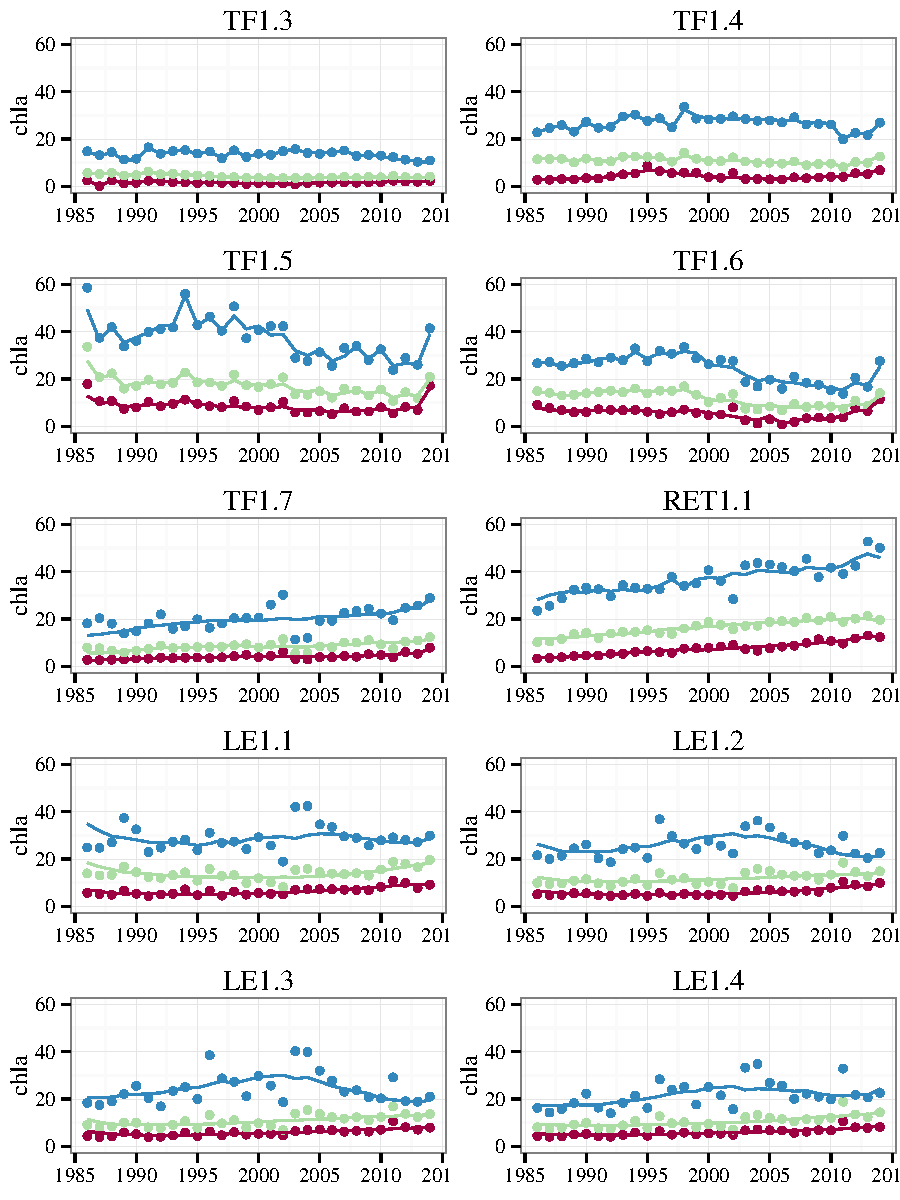
\includegraphics[width = 0.9\textwidth]{figs/patux_prdnrms.pdf}
\caption{Fitted and normalized chlorophyll-a estimates for stations in the Patuxent River estuary using the tidal adaptation of WRTDS.  Colors indicate estimates for the tenth, fiftieth, and ninetieth percentile.}
\label{fig:patux_prdnrms}
\end{figure}

\end{document}
